\documentclass{article}
\usepackage{fancyhdr}
\usepackage{extramarks}
\usepackage{amsmath}
\usepackage{amsthm}
\usepackage{amsfonts}
\usepackage{tikz}
\usepackage[plain]{algorithm}
\usepackage{algpseudocode}

\begin{document}
\author{Chuan Lu}
\title{BIOS:7240 Homework 1}
\maketitle

\medskip

\begin{enumerate}
\item Exercise 1.2

Figure \ref{MSE-MSPE} shows the MSE and MSPE with respect to $p$. It seems as $p$ goes larger, the model becomes more overfitted.
\begin{figure}[htpb]
\centering
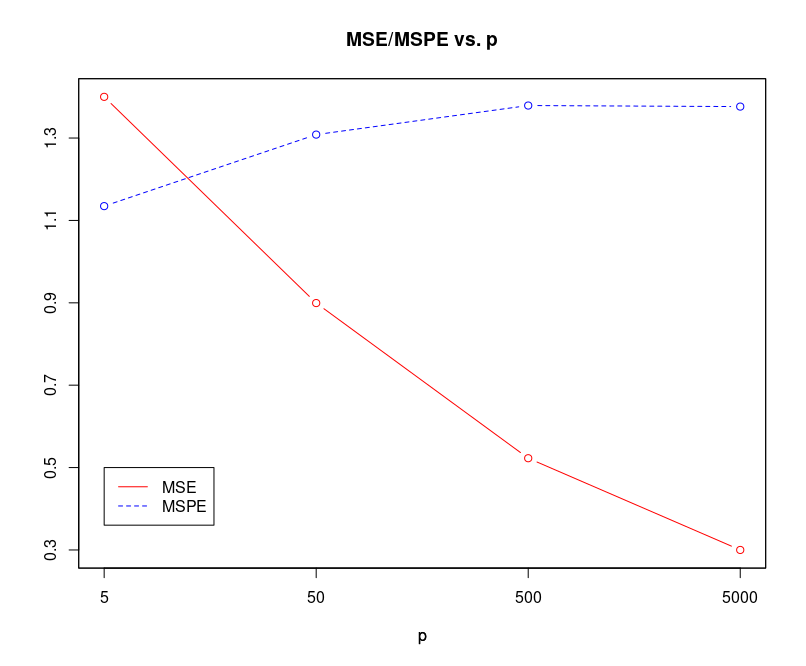
\includegraphics[scale=0.4]{MSE_MSPE.png}
\caption{MSE and MSPE with respect to $p$.}
\label{MSE-MSPE}
\end{figure}

Figure \ref{confint} shows the confidence interval with respect to $p$. 

\begin{figure}[htpb]
\centering
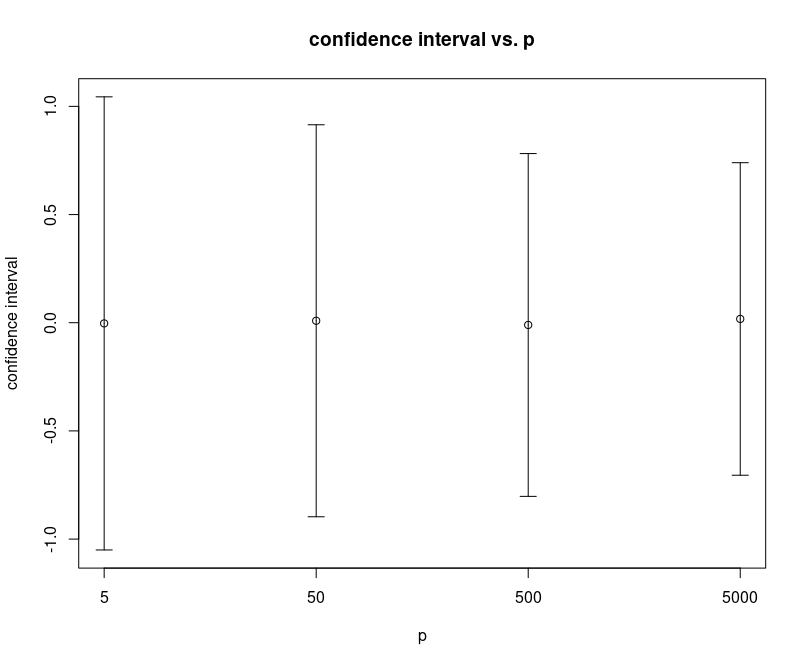
\includegraphics[scale=0.4]{confidence_interval.png}
\caption{Confidence interval with respect to $p$.}
\label{confint}
\end{figure}

\end{enumerate}

\end{document}